\documentclass[tikz,border=8pt]{standalone}
% Shared look for every TikZ diagram. Load with \input{../../tools/tikz-style.tex}
\usepackage[T1]{fontenc}
\usepackage{lmodern}
\renewcommand{\sfdefault}{lmr}  % diagrams use the same serif as the text
\usetikzlibrary{arrows.meta, positioning, shapes.geometric, calc, fit, backgrounds}
\definecolor{cblue}{HTML}{4C78A8}
\definecolor{corange}{HTML}{F58518}
\definecolor{cgreen}{HTML}{54A24B}
\definecolor{cred}{HTML}{E45756}
\definecolor{cpurple}{HTML}{B279A2}
\definecolor{cgrey}{HTML}{6B6B6B}
\tikzset{
  every picture/.style={font=\sffamily, line width=1.2pt},
  box/.style={draw=#1, fill=#1!12, rounded corners=4pt, align=center, inner sep=7pt, minimum height=1.1cm},
  box/.default=cgrey,
  arrow/.style={-{Stealth[length=3mm]}, draw=cgrey, line width=1.4pt},
  title/.style={font=\sffamily\bfseries\Large},
  note/.style={font=\sffamily\small, text=cgrey, align=center},
}
\AtBeginDocument{\hyphenpenalty=10000 \exhyphenpenalty=10000}

% Forward and left directions of a robot at heading 30 deg, as unit arrows in world coordinates.
% Forward = (cos 30, sin 30) = (0.866, 0.5). Left = forward turned by 90 deg = (cos 120, sin 120) = (-0.5, 0.866).
\begin{document}
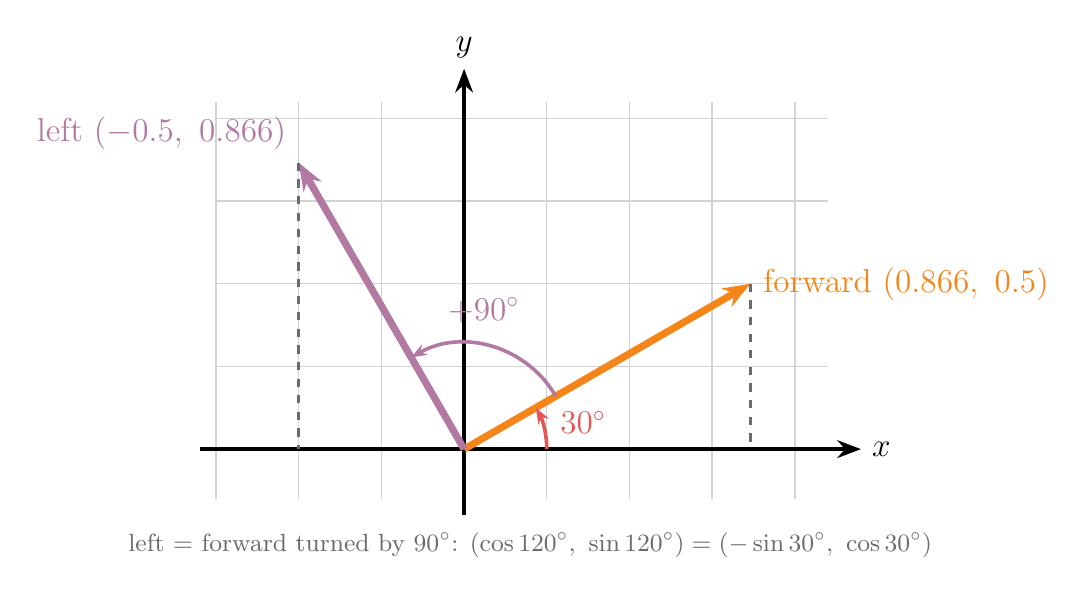
\begin{tikzpicture}[scale=4.2, every node/.append style={font=\large}]
  \draw[cgrey!30, line width=0.5pt] (-0.75,-0.15) grid[step=0.25] (1.1,1.05);
  \draw[arrow, draw=black] (-0.8,0) -- (1.2,0) node[right] {$x$};
  \draw[arrow, draw=black] (0,-0.2) -- (0,1.15) node[above] {$y$};
  \draw[-{Stealth[length=3.5mm]}, corange, line width=2.6pt] (0,0) -- (0.866,0.5) node[right] {forward $(0.866,\ 0.5)$};
  \draw[-{Stealth[length=3.5mm]}, cpurple, line width=2.6pt] (0,0) -- (-0.5,0.866) node[above left] {left $(-0.5,\ 0.866)$};
  \draw[cred, line width=1.3pt, -{Stealth[length=2mm]}] (0.25,0) arc (0:30:0.25);
  \node[cred] at (0.36,0.08) {$30^\circ$};
  \draw[cpurple, line width=1.3pt, -{Stealth[length=2mm]}] ({0.32*cos(30)},{0.32*sin(30)}) arc (30:120:0.32);
  \node[cpurple] at (0.06,0.42) {$+90^\circ$};
  \draw[cgrey, dashed] (0.866,0.5) -- (0.866,0); \draw[cgrey, dashed] (-0.5,0.866) -- (-0.5,0);
  \node[note, anchor=north] at (0.2,-0.22) {left $=$ forward turned by $90^\circ$: $(\cos 120^\circ,\ \sin 120^\circ) = (-\sin 30^\circ,\ \cos 30^\circ)$};
\end{tikzpicture}
\end{document}
